\documentclass[runningheads]{llncs}

\makeatletter
\@ifclassloaded{llncs}{}{%
  \PassOptionsToClass{a4paper,11pt}{article}%
  \LoadClass{article}%
  \usepackage[a4paper,margin=2.4cm]{geometry}}
\makeatother

% ---------------------------------------------------------------------------
%  preamble.tex --- packages, theorem environments and notation macros
% ---------------------------------------------------------------------------
\usepackage[utf8]{inputenc}
\usepackage[T1]{fontenc}
\usepackage{lmodern}
\usepackage{amsmath,amssymb}
% amsthm clashes with llncs (both define proof/theorem); load it only for the
% fallback article class.
\makeatletter
\@ifclassloaded{llncs}{}{\RequirePackage{amsthm}}
\makeatother
\usepackage{booktabs}
\usepackage{graphicx}
\usepackage{caption}
\usepackage{algorithm}
\usepackage{algpseudocode}
\usepackage{microtype}
\usepackage{tikz}
\usetikzlibrary{arrows.meta, positioning, calc, fit, backgrounds,
                shapes.geometric, decorations.pathreplacing, patterns}
\usepackage[hidelinks]{hyperref}
\usepackage[nameinlink]{cleveref}
\usepackage{siunitx}
\sisetup{group-separator={,}, group-minimum-digits=4}

% ---- theorem environments --------------------------------------------------
% llncs already provides theorem, lemma, corollary, proposition, definition,
% remark and proof; the fallback class needs them declared.
\makeatletter
\@ifclassloaded{llncs}{}{%
  \newtheorem{theorem}{Theorem}[section]%
  \newtheorem{lemma}[theorem]{Lemma}%
  \newtheorem{corollary}[theorem]{Corollary}%
  \newtheorem{proposition}[theorem]{Proposition}%
  \newtheorem{definition}[theorem]{Definition}%
  \newtheorem{remark}[theorem]{Remark}%
}
\makeatother

% ---- tikz styles (monochrome) ----------------------------------------------
\tikzset{
  ubox/.style   = {draw=black, thick, align=center, font=\scriptsize,
                   inner sep=3pt, minimum height=5.5mm},
  cell/.style   = {ubox, minimum width=6.5mm, fill=black!5},
  thread/.style = {ubox, minimum width=13mm, fill=black!10},
  stripe/.style = {ubox, minimum width=34mm, fill=white},
  node/.style   = {draw=black, fill=white, minimum width=5mm,
                   minimum height=4mm, inner sep=1pt, font=\tiny},
  dead/.style   = {node, fill=black!25},
  store/.style  = {draw=black, thick, fill=black!5, align=center,
                   font=\scriptsize, inner sep=4pt},
  flow/.style   = {-{Stealth[length=2mm]}, thick},
  read/.style   = {-{Stealth[length=2mm]}, dashed, draw=black!60},
  lbl/.style    = {font=\scriptsize, align=center},
  slbl/.style   = {font=\tiny, align=center},
}

% ---- algorithmic extensions ------------------------------------------------
\algdef{SE}[PARFOR]{ParFor}{EndParFor}[1]%
  {\textbf{parallel for} #1 \textbf{do}}{\textbf{end parallel for}}
\algnewcommand{\Shared}{\textbf{shared-lock}\xspace}
\usepackage{xspace}

% ---- notation --------------------------------------------------------------
\newcommand{\tool}{\textsc{Ptctlmc}}
\newcommand{\uppaal}{\textsc{Uppaal}}
\newcommand{\ltsmin}{\textsc{LTSmin}}
\newcommand{\opaal}{\textsc{opaal}}
\newcommand{\code}[1]{\texttt{\small #1}}

\newcommand{\net}{\mathcal{N}}          % network of timed automata
\newcommand{\clocks}{\mathcal{C}}       % clock set
\newcommand{\dstates}{Q}                % discrete states
\newcommand{\Zone}{Z}                   % a zone
\newcommand{\Passed}{\mathcal{P}}       % passed set
\newcommand{\Frontier}{\mathcal{F}}     % frontier
\newcommand{\succfn}{\mathit{succ}}     % successor function (\succ is a symbol)
\newcommand{\abs}{\alpha}               % aLU abstraction
\newcommand{\subq}{\sqsubseteq}         % subsumption preorder
\newcommand{\hull}{\mathit{hull}}
\newcommand{\mg}{G}                     % minimal constraint system
\newcommand{\extraLU}{\mathit{Extra}^{+}_{LU}}
\newcommand{\stripe}{\mathit{str}}
\newcommand{\zt}{\mathcal{T}}           % zone table
\newcommand{\Covered}{\textsc{Covered}}
\newcommand{\Add}{\textsc{Update}}


\title{Parallelising the Passed Set:\\
  Shared-Memory Zone-Graph Reachability for Timed Automata}
\titlerunning{Parallelising the Passed Set}

\author{PTCTLMC Project}
\authorrunning{PTCTLMC Project}
\institute{Anonymous Submission}

\begin{document}
\maketitle

\begin{abstract}
Zone-graph reachability for timed automata parallelises easily in its successor
function and badly in its passed set, which maintains, per discrete state, a set
of zones under a subsumption preorder: an insertion may drop the candidate,
retire stored zones, or replace stored zones by their convex union.  We present a
shared-memory engine in which threads expand a breadth-first level in parallel
and insert into a passed set striped by discrete state, and in which every
insertion is split into a read-only coverage probe under a shared stripe lock and
the mutating update under an exclusive one.  We prove that coverage is monotone
along every interleaving, which makes a positive probe an exact decision and
yields termination and an interleaving-independent verdict without assuming that
the stored set is an antichain --- an assumption convex merging destroys.  We
then prove that three mechanisms lowering the cost of an update leave the
explored state set unchanged, and bound the work performed at the level barrier.
\end{abstract}

\keywords{Timed automata \and Zone graph \and Parallel model checking \and
          Difference bound matrices \and Subsumption \and Antichains \and OpenMP}

% ---------------------------------------------------------------------------
%  fig_engine --- one breadth-first level of the parallel engine
% ---------------------------------------------------------------------------
\newcommand{\figengine}{%
\begin{figure}[t]
\centering
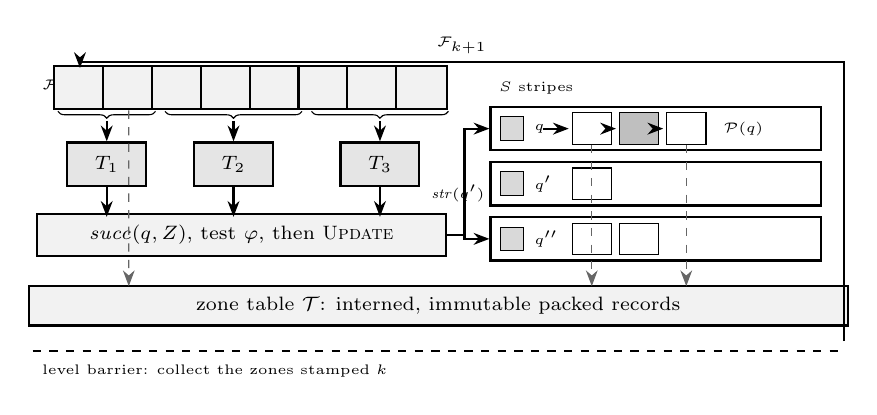
\begin{tikzpicture}[x=1cm, y=1cm]

% ---------------- frontier ------------------------------------------------
\node[slbl, anchor=west] at (-0.45,0.62) {$\Frontier_k$};
\foreach \i in {0,...,7}{\node[cell] (f\i) at ({0.15+0.62*\i},0.62) {};}
\draw[decorate, decoration={brace, amplitude=2.5pt, mirror}] (-0.13,0.32) -- (1.11,0.32);
\draw[decorate, decoration={brace, amplitude=2.5pt, mirror}] (1.23,0.32) -- (2.97,0.32);
\draw[decorate, decoration={brace, amplitude=2.5pt, mirror}] (3.09,0.32) -- (4.83,0.32);

% ---------------- threads --------------------------------------------------
\node[thread, minimum width=10mm] (t1) at (0.49,-0.35) {$T_1$};
\node[thread, minimum width=10mm] (t2) at (2.10,-0.35) {$T_2$};
\node[thread, minimum width=10mm] (t3) at (3.96,-0.35) {$T_3$};
\draw[flow] (0.49,0.20) -- (t1);
\draw[flow] (2.10,0.20) -- (t2);
\draw[flow] (3.96,0.20) -- (t3);

\node[store, minimum width=52mm] (exp) at (2.20,-1.25)
  {$\succfn(q,\Zone)$, test $\varphi$, then \Add};
\draw[flow] (t1) -- (0.49,-1.02);
\draw[flow] (t2) -- (2.10,-1.02);
\draw[flow] (t3) -- (3.96,-1.02);

% ---------------- stripes --------------------------------------------------
\node[slbl, anchor=west] at (5.35,0.62) {$S$ stripes};
\foreach \j/\y in {0/0.10, 1/-0.60, 2/-1.30}{
  \node[stripe, minimum width=42mm, minimum height=5.5mm, anchor=west] (s\j) at (5.35,\y) {};
  \node[draw=black, fill=black!15, minimum width=3mm, minimum height=3mm,
        inner sep=0pt, anchor=west] at (5.48,\y) {};
}
\node[slbl, anchor=west] at (5.80,0.10) {$q$};
\node[node] (n1) at (6.65,0.10) {};
\node[dead] (n2) at (7.25,0.10) {};
\node[node] (n3) at (7.85,0.10) {};
\draw[flow, shorten >=1pt, shorten <=1pt] (5.99,0.10) -- (n1);
\draw[flow, shorten >=1pt, shorten <=1pt] (n1) -- (n2);
\draw[flow, shorten >=1pt, shorten <=1pt] (n2) -- (n3);
\node[slbl, anchor=west] at (8.20,0.10) {$\Passed(q)$};
\node[slbl, anchor=west] at (5.80,-0.60) {$q'$};
\node[node] at (6.65,-0.60) {};
\node[slbl, anchor=west] at (5.80,-1.30) {$q''$};
\node[node] at (6.65,-1.30) {};
\node[node] at (7.25,-1.30) {};

\draw[flow] (exp.east) -- ++(0.22,0) |- (s0.west);
\draw[flow] (exp.east) -- ++(0.22,0) |- (s2.west);
\node[slbl, anchor=south] at (4.95,-0.95) {$\stripe(q')$};

% ---------------- zone table ----------------------------------------------
\node[store, minimum width=104mm] (zt) at (4.70,-2.15)
  {zone table $\zt$: interned, immutable packed records};
\draw[read] (n1) -- (6.65,-1.90);
\draw[read] (n3) -- (7.85,-1.90);
\draw[read] (f1.south) -- (0.77,-1.90);

% ---------------- barrier --------------------------------------------------
\draw[dashed, thick] (-0.45,-2.72) -- (9.85,-2.72);
\node[slbl, anchor=west] at (-0.45,-2.98) {level barrier: collect the zones stamped $k$};
\draw[flow] (9.85,-2.60) -- (9.85,0.95) -- (0.15,0.95) -- (0.15,0.87);
\node[slbl, anchor=south] at (5.0,0.93) {$\Frontier_{k+1}$};

\end{tikzpicture}
\caption{One level: threads claim frontier chunks under a dynamic schedule and
insert each successor into the stripe of its discrete state.  Grey nodes are
retired; dashed edges name zones in $\zt$.}
\label{fig:engine}
\end{figure}}

% ---------------------------------------------------------------------------
%  fig_protocol --- the two-phase stripe protocol
% ---------------------------------------------------------------------------
\newcommand{\figprotocol}{%
\begin{figure}[t]
\centering
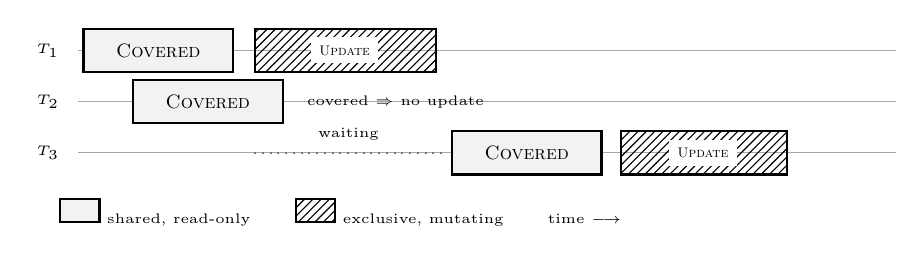
\begin{tikzpicture}[x=1cm, y=1cm]

\foreach \i/\y/\n in {1/0.30/{$T_1$}, 2/-0.35/{$T_2$}, 3/-1.00/{$T_3$}}{
  \node[slbl, anchor=east] at (-0.30,\y) {\n};
  \draw[draw=black!35] (-0.18,\y) -- (10.2,\y);
}

\node[ubox, fill=black!5, minimum width=19mm, anchor=west] at (-0.13,0.30) {\Covered};
\node[ubox, pattern=north east lines, minimum width=23mm, anchor=west] at (2.05,0.30) {};
\node[slbl] at (3.20,0.30) {\colorbox{white}{\Add}};

\node[ubox, fill=black!5, minimum width=19mm, anchor=west] at (0.50,-0.35) {\Covered};
\node[slbl, anchor=west] at (2.60,-0.35) {covered $\Rightarrow$ no update};

\draw[draw=black!55, dotted, thick] (2.05,-1.00) -- (4.45,-1.00);
\node[slbl, anchor=south] at (3.25,-0.96) {waiting};
\node[ubox, fill=black!5, minimum width=19mm, anchor=west] at (4.55,-1.00) {\Covered};
\node[ubox, pattern=north east lines, minimum width=21mm, anchor=west] at (6.70,-1.00) {};
\node[slbl] at (7.75,-1.00) {\colorbox{white}{\Add}};

\node[slbl, anchor=west] at (-0.55,-1.75)
  {\tikz\node[ubox, fill=black!5, minimum width=5mm, minimum height=3mm]{};\
   shared, read-only \qquad
   \tikz\node[ubox, pattern=north east lines, minimum width=5mm, minimum height=3mm]{};\
   exclusive, mutating \qquad time $\longrightarrow$};

\end{tikzpicture}
\caption{The two-phase protocol on one stripe: probes overlap, and only a failed
probe is followed by an update.}
\label{fig:protocol}
\end{figure}}


\section{Introduction}\label{sec:intro}

Establishing the correctness of safety-critical software is a central concern of
formal verification, for which model checking is the established
approach~\cite{Baier08,Clarke99}.  For real-time systems, where correctness
depends not only on functional behaviour but also on timing, software is
typically modelled as a timed automaton~\cite{AlurDill94} and verified against
requirements expressed in Timed Computation Tree
Logic~\cite{AlurCourcoubetisDill90}, as exemplified by industrial case studies
such as the schedulability analysis of the Herschel-Planck satellite
system~\cite{Mikucionis10}.
% TODO: add your own further case-study citations here.

Several tools support this process~\cite{Bozga98,Herbreteau13}, and the one that
has gained the most traction in academia and industry is
\uppaal{}~\cite{Larsen97,Behrmann04}.  Alongside its interface, \uppaal{}
provides an engine for checking timed automata against timed-CTL specifications
that is the state of the art for verifying real-time systems.

As the models to be checked grow, more effective techniques are needed.  The
answer in the past was more powerful hardware, and that answer no longer applies:
processor clock speeds have not increased appreciably in recent years, while core
counts have, and a sequential search cannot use the additional cores.  The
question is therefore what part of a zone-graph search admits parallel execution.

One part admits it directly.  The search explores symbolic states $(q,\Zone)$
pairing a discrete state $q$ with a zone $\Zone$ represented as a difference
bound matrix~\cite{Dill89}, and the successor function $\succfn$ that generates
them is pure: it reads the network and one symbolic state, allocates its result,
and touches no shared data.  Calls on distinct symbolic states are independent,
and a level-synchronous breadth-first search exposes that independence.  The
passed set, which stores what the search has already seen, is the part that does
not, and it differs from the explicit-state case in three ways that together
decide the design of an engine.  It stores, per discrete state, a set of zones
maintained under a subsumption preorder~\cite{Behrmann06,Herbreteau12}, so
inserting a zone may drop it, retire stored zones, or replace stored zones by a
convex union: the operation writes as well as reads, and insert-if-absent, which
a lock-free shared hash table implements directly~\cite{Laarman10}, does not
describe it.  Its effect depends on the order in which zones arrive, so the set
of stored zones is not a function of the reachable set and no scheduling
discipline makes it one.  And each call is expensive, because stored zones are
kept as minimal constraint systems~\cite{LarsenLPY97} while the zone algebra
needs dense canonical matrices.

This paper presents a shared-memory engine organised around those three
properties.  Threads expand one breadth-first level in parallel and insert
successors directly into a passed set striped by discrete state, so expansion and
insertion are fused.  Each insertion is split in two: a read-only coverage probe
under a shared stripe lock, and the mutating update under an exclusive one.  The
split is worth having only if a positive probe remains valid after the lock is
released, and that is the technical core of the paper: coverage is monotone along
every interleaving, so a probe is an exact decision for the case it answers
rather than an observation a second phase must validate.  The same property does
the rest of the work.  It bounds the number of insertions at a discrete state by
the number of abstraction classes, which gives termination and an
interleaving-independent verdict without assuming that the stored set is an
antichain --- an assumption convex merging destroys and that termination
arguments for subsumption-based searches normally rest on.

Three further mechanisms reduce the cost of one update and are each proved not to
change which symbolic states are explored: inclusion decided directly against the
stored minimal constraint system, a dense mirror of a stored set admitted on
accumulated query work rather than on size, and a bounded convex-union window.
Three more bound the work at the level barrier, which is the engine's only serial
term and the one that grows with the state space: a bucketed collection of the
next frontier, an incrementally triggered compaction of retired nodes, and a
growth-triggered reclamation of the shared zone table that is amortised $O(1)$
per interned zone and keeps unreclaimed garbage below the live set.

\Cref{sec:prelim} fixes notation and the three properties of subsumption the
proofs use, \cref{sec:approach} describes the engine, \cref{sec:correct} proves
it correct and bounds the cost of each mechanism, \cref{sec:related} places it
against related work, and \cref{sec:eval} evaluates it.

\section{Preliminaries}\label{sec:prelim}

\paragraph{Networks and the zone graph.}
A network $\net$ of timed automata~\cite{AlurDill94} is a parallel composition of
finite automata over a set of real-valued clocks $\clocks$, shared bounded
integer variables, and synchronisation channels; edges carry clock guards, resets
and integer updates, locations carry invariants.  A \emph{discrete state} $q$ is
the tuple of current locations together with the values of the integer variables;
$\dstates$ is the finite set of discrete states.  A \emph{zone} is a set of clock
valuations definable by a conjunction of constraints $x_i - x_j \prec c$, where
$x_0$ is the reference clock, constantly zero.  A \emph{symbolic state} is a pair
$(q,\Zone)$ with $\Zone$ non-empty.  The \emph{successor function}
$\succfn(q,\Zone)$ applies one edge, or one synchronised pair or broadcast of
edges: it conjoins guards, applies resets and integer updates, lets time elapse
subject to the invariants of the target locations, and discards empty results.
It reads only $\net$ and its argument and allocates its result, so it is pure.
Given a predicate $\varphi$ on symbolic states, the question is whether some
$(q,\Zone)$ with $\varphi(q,\Zone)$ is reachable from $(q_0,\Zone_0)$.

\paragraph{Zones as matrices.}
A zone over $n$ clocks is stored as a difference bound matrix
(DBM)~\cite{Dill89,Bengtsson04}: entry $\Zone[i][j]$ is the tightest known bound
on $x_i - x_j$, drawn from a set of bounds ordered by strength and closed under
addition.  A DBM is \emph{canonical} when $\Zone[i][j] \le \Zone[i][k] +
\Zone[k][j]$ for all $i,j,k$; canonicity is restored by an all-pairs
shortest-path closure at cost $O(n^3)$, and all DBMs here are canonical.
Canonicity makes inclusion entrywise,
\begin{equation}\label{eq:denseincl}
  \Zone \subseteq \Zone' \iff \forall i,j:\ \Zone[i][j] \le \Zone'[i][j],
\end{equation}
and makes the entrywise maximum $\hull(\Zone,\Zone')$ --- the smallest zone
containing both --- canonical as well.  We say $\Zone$ and $\Zone'$ \emph{merge
exactly} when $\Zone \cup \Zone' = \hull(\Zone,\Zone')$, so that replacing the
pair by the hull loses and gains nothing.

A \emph{minimal constraint system} $\mg(\Zone)$ is a set of difference
constraints with $\mathrm{close}(\mg(\Zone)) = \Zone$ containing no redundant
constraint~\cite{LarsenLPY97}; it has $O(n)$ constraints on the models we
consider, against $O(n^2)$ matrix entries.  Its byte encoding is the
\emph{packed record} of $\Zone$, and \emph{unpacking} is the $O(n^3)$ closure
that rebuilds the canonical matrix from it.

\paragraph{Subsumption.}
A search need not store a symbolic state whose behaviour a stored one already
covers.  Which states those are is fixed by a preorder on zones, and the engine
uses one of two.  The first is inclusion.  The second is the abstraction
$\abs_q$ induced by the $\preceq_{LU}$ preorder on
valuations~\cite{Behrmann06,Herbreteau12}: with $L_q(x)$ and $U_q(x)$ the largest
constants against which clock $x$ is compared by a lower, respectively upper,
guard reachable from $q$, floored by the constants of $\varphi$, the relation $v
\preceq_{LU} v'$ holds when no guard within those bounds separates $v$ from $v'$,
and $\abs_q(\Zone)$ is the downward closure of $\Zone$ under it.  We write
\begin{equation}\label{eq:alu}
  \Zone \subq_q \Zone' \quad:\iff\quad \Zone \subseteq \abs_q(\Zone'),
\end{equation}
decidable entrywise on canonical DBMs in $O(n^2)$~\cite{Herbreteau12}, reading
arbitrary entries of $\Zone'$.  The engine uses \cref{eq:alu} by default and
inclusion when $\varphi$ constrains clocks or the network contains diagonal
constraints, both of which make $\abs_q$ unsound.  We write $\subq_q$ for
whichever is in force; every result below holds for both.  Given a passed set
$\Passed$ mapping each $q$ to its \emph{stored set} $\Passed(q)$, a symbolic
state is \emph{covered}, written $\mathrm{cov}_\Passed(q,\Zone)$, when some
$Y \in \Passed(q)$ satisfies $\Zone \subq_q Y$.

Three properties of $\subq_q$ are used throughout.

\begin{lemma}[Preorder]\label{lem:preorder}
$\subq_q$ is reflexive and transitive, and $\Zone \subseteq \Zone'$ implies
$\Zone \subq_q \Zone'$.
\end{lemma}
\begin{proof}
$\preceq_{LU}$ is reflexive and transitive, so its downward closure $\abs_q$ is
extensive, monotone and idempotent, i.e.\ a closure operator.  Reflexivity is
extensivity.  If $\Zone \subseteq \abs_q(\Zone')$ and $\Zone' \subseteq
\abs_q(\Zone'')$ then $\abs_q(\Zone) \subseteq \abs_q(\abs_q(\Zone')) =
\abs_q(\Zone') \subseteq \abs_q(\abs_q(\Zone'')) = \abs_q(\Zone'')$, and $\Zone
\subseteq \abs_q(\Zone)$ gives transitivity.  The last claim is monotonicity
followed by extensivity.  For inclusion all three are immediate.\qed
\end{proof}

\begin{lemma}[Simulation]\label{lem:sim}
If $\Zone \subq_q \Zone'$ then every $(q',\Zone_1) \in \succfn(q,\Zone)$ has a
counterpart $(q',\Zone_2) \in \succfn(q,\Zone')$ with $\Zone_1 \subq_{q'}
\Zone_2$; and $\varphi(q,\Zone)$ implies $\varphi(q,\Zone')$.
\end{lemma}

\begin{lemma}[Finite index]\label{lem:finite}
For each $q$, the set $\{\abs_q(\Zone) : \Zone \text{ a zone}\}$ is finite.
\end{lemma}

\Cref{lem:sim} is the defining property of a sound subsumption relation, proved
for $\abs_q$ in~\cite{Behrmann06,Herbreteau12} and immediate from monotonicity of
the DBM operations for inclusion; its second half is what forces the fallback to
inclusion when $\varphi$ reads clocks, since $\abs_q$ may drop concrete
valuations.  \Cref{lem:finite} is standard~\cite{Behrmann06}.  Under inclusion
the corresponding finiteness comes instead from \emph{extrapolation}:
$\extraLU(\Zone)$ widens $\Zone$ to a representative from a finite
set~\cite{Daws98,Behrmann06}, at the price of a coarser zone.

\section{The Engine}\label{sec:approach}

The engine is a level-synchronous breadth-first search over the zone graph in
which every thread inserts into one shared passed set.  We describe it bottom-up:
first the passed set and the operation a thread performs on it, then the parallel
level loop that calls that operation and the protocol under which it is called,
then the work that runs at a level barrier.  Correctness and cost bounds are
deferred to \cref{sec:correct}; this section states what the engine does and why
each mechanism is there.

\subsection{The passed set and its update}\label{sec:passed}

The passed set is one structure that every thread may touch, partitioned into $S$
\emph{stripes} by a hash of the discrete state.  A stripe owns a lock, a slot
table mapping a discrete state to the head of a chain, and the chain nodes
themselves; a node holds the index of one stored zone and the breadth-first level
at which it was stored.  Since $\stripe$ is a function of the discrete state, all
updates at one discrete state take one lock, and updates at discrete states in
different stripes touch disjoint memory.

Zones are not held in the chains.  All distinct zones live in one \emph{zone
table} $\zt$ shared by every stripe, which stores each zone once as a packed
record and hands out an index; chain nodes and frontier entries hold indices.
Interned records are immutable while referenced, because every operation below
mutates only the incoming zone and reads stored ones, so reads take no lock and
only the first sight of a distinct zone takes one.

\begin{algorithm}[t]
\caption{The stored-set update and the coverage probe at one discrete state}
\label{alg:update}
\begin{algorithmic}[1]
\Procedure{Update}{$q,\Zone,k$} \Comment{exclusive lock on $\stripe(q)$ held}
  \If{$\exists\, Y \in \Passed(q):\ \Zone \subseteq \mg(Y)$}
      \Return \textsc{dropped} \Comment{on the packed records}
  \EndIf
  \State $A \leftarrow \Passed(q)$ as dense matrices, newest first
         \Comment{mirror, else one unpack each}
  \If{$\exists\, Y \in A:\ \Zone \subq_q Y$} \Return \textsc{dropped}
      \Comment{(a)} \EndIf
  \State retire $\{Y \in A : Y \subq_q \Zone\}$ and remove it from $A$
         \Comment{(b)}
  \While{some $Y$ among the $m$ newest of $A$ merges exactly with $\Zone$}
    \State $\Zone \leftarrow \hull(\Zone,Y)$; retire $Y$ and remove it from $A$
           \Comment{(c)}
  \EndWhile
  \State intern $\Zone$, add it to $\Passed(q)$ stamped $k$, maintain the mirror
  \State \Return \textsc{inserted}
\EndProcedure
\Statex
\Procedure{Covered}{$q,\Zone$} \Comment{shared lock on $\stripe(q)$ held; writes nothing}
  \If{$\Passed(q)$ has a mirror}
      \Return $\exists\, Y \in \Passed(q):\ \Zone \subq_q Y$ \EndIf
  \State \Return $\exists\, Y \in \Passed(q):\ \Zone \subseteq \mg(Y)$
\EndProcedure
\end{algorithmic}
\end{algorithm}

\Cref{alg:update} states the two procedures a thread calls per successor, where
$\Passed(q)$ ranges over live zones only.  \textsc{Update} is the operation the
search needs: fold~(a) drops the candidate $\Zone$ when a stored zone subsumes
it, fold~(b) retires the stored zones that $\Zone$ subsumes, and fold~(c) absorbs
stored zones that merge exactly with $\Zone$, replacing $\Zone$ by the hull and
repeating, because a hull can merge with a zone the original could not.  What
survives is interned and added.  \textsc{Covered} is the read-only prefix of that
operation: it decides fold~(a) and writes nothing.

Three parts of \cref{alg:update} exist to keep the cost of one call low, and each
is stated here and justified in \cref{sec:cost}.

\emph{The packed-record filter, line~2.}  Every predicate in folds (a)--(c) reads
a stored zone as a dense matrix, and stored zones are packed records, so a direct
implementation unpacks a record per probe at cost $O(n^3)$.  A minimal constraint
system is a generating set, and inclusion can be decided against generators
without rebuilding what they generate: $\Zone \subseteq \mathrm{close}(\mg)$
holds exactly when $\Zone[i][j] \le b$ for every $(i,j,b) \in \mg$.  Line~2 runs
that test, which costs $O(|\mg|)$ and needs no scratch matrix.  A hit ends the
call; a miss falls through to the unchanged folds.  \textsc{Covered} uses the
same test, and only that test, when the stored set has no mirror.

\emph{The dense mirror.}  Where line~2 does not fire, the folds read every live
zone densely, so an update costs $\Theta(L \cdot n^3)$ for a stored set of $L$
live zones.  Stored sets of size close to one, the common case on process
networks, pay little; stored sets that grow do not, and a model of one automaton
with one location and $N$ independent clocks keeps its entire passed set in a
single stored set of thousands of mutually incomparable zones.  Such a stored set
additionally keeps its live zones as dense canonical matrices in insertion order,
in a \emph{dense mirror} that the folds read in place.  The packed records remain
the storage of record; the mirror is a cache, appended on insertion, its slot
cleared on retirement, rebuilt when half its slots are cleared, and subject to a
byte budget that may refuse to create it.  It is created once the unpacking the
stored set has already cost crosses a threshold: with $v$ the number of updates
that have walked it, when $v \cdot L \ge W$ and $L \ge L_{\min}$.  What a mirror
saves is one unpack per live zone \emph{per visit}, so the product governs it and
a rule on $L$ alone cannot see the difference between $16$ zones walked $100$
times and $64$ walked once.  The floor $L_{\min}$ is a memory condition: a mirror
of a one-zone stored set is a private copy of a zone the zone table was sharing.

\emph{The merge window $m$.}  Fold~(c) restarts after each success, so its cost is
quadratic in $L$ --- and it is quadratic exactly where stored sets are large.  A
candidate therefore attempts to merge only with the $m$ most recently inserted
live zones.  Zones that merge are almost always recent neighbours, because a
merge happens when a successor extends a zone stored moments earlier.

\subsection{Parallel level-synchronous exploration}\label{sec:levels}

\figengine

A search that interleaves a call to $\succfn$ with the update of its result
serialises, because the update performed for one successor is observed by the
check performed for the next.  Grouping the search by breadth-first level breaks
that dependency for the calls to $\succfn$.  The \emph{frontier} $\Frontier_k$ is
the set of symbolic states inserted during level $k$; every one of them was
checked against the passed set before being placed there, so their expansions are
independent and may run in any order.  A frontier entry is a (discrete state,
zone index) pair: its zone is read from $\zt$ when the entry is expanded, rather
than copied into the frontier, so the frontier does not hold a second copy of
zones the passed set already stores.

\Cref{alg:engine} states one level and \cref{fig:engine} shows it.  Threads claim
chunks of the frontier under a dynamic schedule and insert each successor into
the stripe of its discrete state as soon as it is generated.  Fusing expansion
and insertion removes a second pass over data that has just left cache, and it
lets every thread see, within a level, the zones the others have stored.

\begin{algorithm}[t]
\caption{One level of the parallel engine}
\label{alg:engine}
\begin{algorithmic}[1]
\Require network $\net$, predicate $\varphi$, thread count $T$, stripe count $S \gg T$
\State $\Passed(q_0) \leftarrow \{\Zone_0\}$;\enspace
       $\Frontier \leftarrow [(q_0,\Zone_0)]$;\enspace $k \leftarrow 0$
\While{$\Frontier \neq \emptyset$}
  \State $k \leftarrow k+1$
  \ParFor{$i = 0,\dots,|\Frontier|-1$} \Comment{dynamic schedule}
    \State $(q,\Zone) \leftarrow$ decode $\Frontier[i]$
    \ForAll{$(q',\Zone') \in \succfn(q,\Zone)$}
      \If{$\varphi(q',\Zone')$} \Return \textbf{true} \EndIf
      \State \textbf{lock} $\stripe(q')$ \textbf{shared};\enspace
             $c \leftarrow \Covered(q',\Zone')$;\enspace \textbf{unlock}
      \If{$c$} \textbf{continue} \EndIf
      \State \textbf{lock} $\stripe(q')$ \textbf{exclusive};\enspace
             $r \leftarrow \Add(q',\Zone',k)$;\enspace \textbf{unlock}
      \If{$r = \textsc{inserted}$} record $q'$ in this thread's touched set \EndIf
    \EndFor
  \EndParFor
  \State $\Frontier \leftarrow$ zones stamped $k$ of the touched discrete states
  \State compact retired nodes; reclaim unreferenced records of $\zt$; revise the abstraction
\EndWhile
\Return \textbf{false}
\end{algorithmic}
\end{algorithm}

Two details of \cref{alg:engine} are load-bearing for \cref{sec:correct}.  The
predicate $\varphi$ is evaluated on \emph{generated} symbolic states, on line~7,
and never on a stored zone, so a zone that fold~(c) built as a convex union is
never offered to it.  And a thread records the discrete states it inserted into
rather than the states themselves; the next frontier is read back out of the
passed set at the barrier, so a zone inserted early in a level and retired later
in the same level does not enter it.

\paragraph{The two-phase stripe protocol.}
Lines~8--11 split the operation of \cref{alg:update} into its read-only and its
mutating half.  \textsc{Covered} runs under a \emph{shared} stripe lock, so
probes issued by different threads on one stripe proceed concurrently, and only a
thread whose probe answers \emph{no} takes the \emph{exclusive} lock and runs
\textsc{Update} (\cref{fig:protocol}).  The split pays because the operation is
read-mostly and because collisions are structural rather than random: a successor
is routed to the stripe of its discrete state, and a symmetric network sends many
successors of one level to the same discrete state, hence to one stripe.  It is
sound because a positive probe cannot be invalidated while the shared lock is
released, which is \cref{lem:monotone}.  A probe answering \emph{no} where
\textsc{Update} would have dropped the candidate costs one exclusive lock and
nothing else, since \textsc{Update} repeats the test.

\figprotocol

Critical sections here last microseconds, so each stripe carries an eight-byte
reader/writer lock that spins a bounded number of times before yielding, with the
bound set from the thread count relative to the core count.

\paragraph{The interface to the correctness argument.}
\Cref{sec:correct} uses the update only through the following contract.  Write
$\Passed(q)$ for the stored set before an update with candidate $\Zone$ at $q$,
and $\Passed'(q)$ for the stored set after it.
\emph{(U1)} If $\mathrm{cov}_\Passed(q,\Zone)$ then $\Passed'(q) = \Passed(q)$
and nothing is recorded as inserted.
\emph{(U2)} Otherwise $\Passed'(q) = \{\Zone^{*}\} \cup (\Passed(q) \setminus R)$
for some $R \subseteq \Passed(q)$ and some $\Zone^{*}$ with $\Zone \subseteq
\Zone^{*} \subseteq \Zone \cup \bigcup R$ and $Y \subq_q \Zone^{*}$ for every $Y
\in R$.
\emph{(U3)} All updates at one discrete state are totally ordered, and each
observes the stored set left by its predecessor.

\subsection{The level barrier}\label{sec:barrier}

Expansion is parallel and contended only where discrete states collide, so
whatever runs between levels is the engine's serial term, and it touches the
passed set, which is larger at every level.  Four things run there.

\emph{Collecting the next frontier.}  The next frontier is the set of zones
stamped with the level just finished, read out of the passed set over the
discrete states the threads recorded.  A discrete state may be recorded by
several threads and must be scanned once, so the records are deduplicated: the
keys are partitioned by a hash into $B$ buckets and each bucket is deduplicated
and scanned independently, in one parallel pass.  The bucket function is taken
from the same hash as $\stripe$, so a bucket owns a contiguous range of stripes
and its scan stays within one slice of the passed set.

\emph{Compacting retired nodes.}  Folds (b) and (c) retire chain nodes by marking
them, because unlinking while other threads hold chain positions is not safe
during a level.  Marked nodes are traversed and skipped by every later chain walk,
so they are removed between levels, one thread per stripe, by rebuilding each
chain from its live nodes.  A stripe is rebuilt once its marked nodes reach a
third of its nodes, and that count is maintained incrementally by the two sites
that retire a node rather than recomputed by a scan, so the trigger is $O(1)$ and
can be evaluated at every barrier.

\emph{Reclaiming the zone table.}  A retired node may hold the last reference to
an interned record.  Unreferenced records are reclaimed by marking every record
named by a live chain node or by a frontier entry --- the frontier is a root ---
and returning the rest to a free list.  The trigger is growth-based.  Let $A$ be
the number of records currently handed out, that is the high-water index count
minus the size of the free list; $A$ rises with every fresh intern and falls back
to the live set after a reclamation, so it is the quantity a trigger must watch.
A reclamation runs when $A \ge \mathit{next}$, after which $\mathit{next}
\leftarrow \max(2A_{\mathrm{live}}, \tau)$ for a floor $\tau$ below which the
scan is not worth its own cost.  Freed records and freed indices are recycled in
place, so no index held by a chain node is ever renumbered; the price is that
every memo mapping record content to an index, or an index to a decoded matrix,
must be invalidated, which the engine does by stamping each memo with a
reclamation counter.

\emph{Revising the abstraction.}  Subsumption and extrapolation are two routes to
finiteness and they act differently: $\subq_q$ only prunes, dropping a zone when
a stored one simulates it, whereas $\extraLU$ widens, mapping many zones onto one
representative.  Where the reachable zones at a discrete state are mutually
$\subq_q$-incomparable, pruning achieves nothing and widening collapses them;
where they collapse under $\subq_q$ anyway, widening only costs precision.  Which
case holds is a property of the model, and the distinguishing signal is available
in $O(1)$ per stripe at a barrier: the ratio of live stored zones to distinct
discrete states, near one when subsumption is collapsing the stored sets and
climbing when they fill with incomparable zones.  The engine therefore starts
without extrapolation and switches it on, for every zone generated thereafter, at
the first barrier at which the ratio crosses a threshold $\theta$.  The switch is
monotone, so a run performs at most one.

\section{Correctness and Cost}\label{sec:correct}

The engine has two obligations that do not follow from the standard argument for
a subsumption-based search: it must terminate although convex merging destroys
the antichain property, and its verdict must be the correct one although its
stored set depends on the schedule.  We discharge both from a single property of
the update, which also justifies the two-phase protocol, and then bound the cost
of each mechanism of \cref{sec:approach}.

\subsection{The contract and the probe}

\begin{proposition}\label{prop:contract}
\textsc{Update} of \cref{alg:update} satisfies \emph{(U1)--(U3)}, for every
merge window $m \ge 0$ and whether or not the stored set has a mirror.
\end{proposition}
\begin{proof}
\emph{(U1).}  The procedure returns \textsc{dropped} without mutating anything
exactly when line~2 or fold~(a) fires.  Fold~(a) tests $\Zone \subq_q Y$ over
every live stored zone, so it fires whenever $\mathrm{cov}_\Passed(q,\Zone)$
holds; line~2 fires only when $\Zone \subseteq Y$ for some live $Y$, which
implies $\Zone \subq_q Y$ by \cref{lem:preorder}, so adding it neither creates
nor removes drops.  Conversely a drop exhibits a stored $Y$ with $\Zone \subq_q
Y$, so coverage held.

\emph{(U2).}  Let $R$ be the set of zones retired by folds~(b) and~(c) and
$\Zone^{*}$ the zone finally interned.  Fold~(c) replaces the current candidate
$Y_t$ by $\hull(Y_t,Y'_t)$, which equals $Y_t \cup Y'_t$ because the merge
condition requires the union to be exact, and retires $Y'_t$; after $r$ merges
$\Zone^{*} = \Zone \cup Y'_1 \cup \dots \cup Y'_r$.  Hence $\Zone \subseteq
\Zone^{*} \subseteq \Zone \cup \bigcup R$, and each $Y'_t \subseteq \Zone^{*}$
gives $Y'_t \subq_q \Zone^{*}$ by \cref{lem:preorder}.  A zone $Y$ retired by
fold~(b) satisfies $Y \subq_q \Zone \subseteq \Zone^{*}$, so $Y \subq_q
\Zone^{*}$ by \cref{lem:preorder} and transitivity.  Both arguments are
independent of how many merges were attempted, so they hold for every $m$; and
they read stored zones only, which is what a mirror changes.

\emph{(U3).}  Every call at $q$ holds the exclusive lock of $\stripe(q)$, and
$\stripe$ is a function of $q$.\qed
\end{proof}

\begin{lemma}[Monotonicity of coverage]\label{lem:monotone}
Let $\Passed$ and $\Passed'$ be the stored sets at $q$ before and after one
update.  Then $\mathrm{cov}_\Passed(q,X)$ implies $\mathrm{cov}_{\Passed'}(q,X)$
for every zone $X$.  Consequently, along every interleaving, once a symbolic
state is covered it stays covered.
\end{lemma}
\begin{proof}
Let $Y \in \Passed(q)$ with $X \subq_q Y$.  Under (U1) the stored set is
unchanged.  Under (U2), either $Y \notin R$, so $Y \in \Passed'(q)$; or $Y \in
R$, so $Y \subq_q \Zone^{*} \in \Passed'(q)$ and transitivity
(\cref{lem:preorder}) gives $X \subq_q \Zone^{*}$.  The second statement follows
by induction over the sequence of updates at $q$, which is well defined by
(U3).\qed
\end{proof}

\Cref{lem:monotone} does not say that the stored set grows: zones are retired and
its size can fall.  It says that the set of covered symbolic states grows, which
is the only thing a coverage probe reports on.

\begin{theorem}[The probe is exact for the case it answers]\label{thm:probe}
If a thread's probe at $(q,\Zone)$ returns \emph{true} and the thread skips the
update, the resulting passed set and the set of states recorded as inserted are
identical to those obtained by running the update at any later point of the same
interleaving.
\end{theorem}
\begin{proof}
The probe holds the shared lock of $\stripe(q)$, which excludes every writer of
that stripe, so it reads one well-defined stored set $\Passed_t(q)$, and
returning \emph{true} means $\mathrm{cov}_{\Passed_t}(q,\Zone)$.  For any later
$t'$, \cref{lem:monotone} gives $\mathrm{cov}_{\Passed_{t'}}(q,\Zone)$, so an
update executed at $t'$ takes branch (U1): it leaves the stored set unchanged and
records nothing, which is what skipping does.\qed
\end{proof}

\Cref{thm:probe} separates this protocol from optimistic concurrency, which reads
without exclusion, acts, and re-validates because its observation may have been
invalidated.  Here a positive observation cannot be invalidated, so there is
nothing to re-validate and the mutating phase is not entered at all.

\subsection{Termination and verdict}

\begin{theorem}\label{thm:term}
Assume the candidates offered at each discrete state $q$ fall into finitely many
classes of $\Zone \equiv_q \Zone' :\iff \abs_q(\Zone) = \abs_q(\Zone')$.  Then
the engine performs finitely many insertions and terminates, for every
interleaving.
\end{theorem}
\begin{proof}
Fix $q$ and let $\Zone_1,\Zone_2,\dots$ be the candidates inserted at $q$ in the
total order given by (U3).  Suppose $\Zone_i \equiv_q \Zone_j$ for some $i < j$.
Then $\Zone_j \subseteq \abs_q(\Zone_j) = \abs_q(\Zone_i)$, i.e.\ $\Zone_j
\subq_q \Zone_i$.  Immediately after the insertion of $\Zone_i$ the stored set
contains $\Zone_i^{*} \supseteq \Zone_i$, so $\mathrm{cov}(q,\Zone_i)$ held then,
and by \cref{lem:monotone} it still holds when $\Zone_j$ is offered: there is a
stored $Y$ with $\Zone_i \subq_q Y$, hence $\Zone_j \subq_q Y$ by transitivity,
so the update of $\Zone_j$ takes branch (U1) and does not insert --- contradicting
the choice of $\Zone_j$.  The inserted candidates therefore lie in pairwise
distinct classes, and their number is bounded by the number of classes at $q$.
Summing over the finite set $\dstates$ bounds the total number of insertions.
The frontier of level $k+1$ consists of zones inserted during level $k$, so a
level that inserts nothing ends the search; the number of levels is therefore
finite and each expands a finite frontier.\qed
\end{proof}

The hypothesis holds in both subsumption modes: under \cref{eq:alu} by
\cref{lem:finite}, and under inclusion because every candidate is then
$\extraLU$-extrapolated and those form a finite set~\cite{Daws98,Behrmann06}.
The proof uses neither an antichain invariant nor any order on updates beyond
(U3).  This is what makes it survive fold~(c), which can leave a stored $Y$ with
$Y \subq_q \Zone^{*}$ un-retired, and parallel execution, which fixes no order
across discrete states.

\begin{lemma}[Exact unions are transparent to $\succfn$]\label{lem:union}
If $Y = \Zone_1 \cup \Zone_2$ as sets of valuations, then for every edge, or
synchronised pair of edges, of $\net$ the zone produced from $Y$ is the union of
the zones produced from $\Zone_1$ and from $\Zone_2$.
\end{lemma}
\begin{proof}
The successor computation composes conjunction with a guard or invariant, clock
reset, and time elapse.  Each is defined pointwise on valuations --- $\{v : v
\models g\} \cap S$, $\{v[x{:=}0] : v \in S\}$ and $\{v + d : v \in S, d \ge 0\}$
--- and every operation of that shape commutes with union.\qed
\end{proof}

\begin{proposition}\label{prop:sound}
At every point of every interleaving, every $Y \in \Passed(q)$ satisfies $Y
\subseteq \bigcup\{\Zone : (q,\Zone) \text{ reachable}\}$.
\end{proposition}
\begin{proof}
Induction over the updates in the order given by (U3).  Initially $\Passed(q_0) =
\{\Zone_0\}$.  Branch (U1) changes nothing.  Branch (U2) adds $\Zone^{*}
\subseteq \Zone \cup \bigcup R$, where $\Zone$ is the zone of a generated
symbolic state and each $Y \in R$ satisfies the claim by hypothesis; by
\cref{lem:union} and the hypothesis, every generated zone at $q$ is contained in
the union of the reachable zones at $q$.\qed
\end{proof}

\begin{theorem}\label{thm:verdict}
For every interleaving, the engine returns \emph{true} if and only if some
reachable symbolic state satisfies $\varphi$.
\end{theorem}
\begin{proof}
\emph{Soundness.}  The engine returns \emph{true} only after evaluating $\varphi$
on a generated symbolic state $(q,\Zone_g)$; stored zones are never offered to
$\varphi$.  By \cref{lem:union,prop:sound}, $\Zone_g$ lies in the union of the
zones of reachable symbolic states at $q$.  As $\varphi$ is a condition on $q$
conjoined with a clock constraint tested for non-empty intersection, a witness
inside that union is a witness inside one of its operands.

\emph{Completeness.}  A zone inserted during level $j$ is stamped $j$ and, if
still live at the barrier of level $j$, is collected into $\Frontier_{j+1}$ and
expanded during level $j+1$; so at termination every live stored zone has been
expanded, the final frontier being empty.  Let $(q,\Zone)$ be reachable with
$\varphi(q,\Zone)$; we induct on the length $d$ of a path to it.  For $d = 0$ the
initial state is tested explicitly.  For $d > 0$ write $(q,\Zone) \in
\succfn(q_p,\Zone_p)$.  A second induction on $d$ shows
$\mathrm{cov}_\Passed(q_p,\Zone_p)$ at termination: the candidate covering
$(q_p,\Zone_p)$ was either dropped, in which case coverage held then and still
holds by \cref{lem:monotone}, or inserted, in which case coverage held
immediately after.  Let $Y_p$ be a witness; it was expanded, and \cref{lem:sim}
gives $(q,\Zone_2) \in \succfn(q_p,Y_p)$ with $\varphi(q,\Zone_2)$.  That
successor was generated and tested.\qed
\end{proof}

\Cref{thm:verdict} is the precise sense in which the engine is deterministic.
The stored set is not: it depends on the order in which candidates reach a
discrete state.  The verdict, and the set of covered symbolic states at
termination, do not.

\begin{proposition}[The abstraction switch is sound mid-run]\label{prop:adaptive}
Enabling $\extraLU$ at a barrier preserves \emph{(U1)--(U3)}, hence
\cref{thm:term,thm:verdict}.
\end{proposition}
\begin{proof}
The switch changes which zone is offered as a candidate and nothing about the
passed-set discipline: the same preorder $\subq_q$ is used before and after, and
the contract refers only to it, so a stored set mixing exact and widened zones is
covered by the same argument as a homogeneous one.  In \cref{thm:verdict},
completeness uses $\Zone \subq_q \Zone_2 \subseteq \extraLU(\Zone_2)$ and
transitivity; soundness needs $\extraLU$ to preserve $\varphi$, which holds
because $L_q$ and $U_q$ are floored by the clock constants of $\varphi$, so
$\varphi$ is preserved for the same reason a guard
is~\cite{Behrmann06,Daws98}.  Termination is unaffected, the switch being enabled
only when $\subq_q$ is \cref{eq:alu}, whose finite index already discharges the
hypothesis of \cref{thm:term}.\qed
\end{proof}

\subsection{What the update's cost mechanisms preserve}\label{sec:cost}

\begin{lemma}[Inclusion against a minimal constraint system]\label{lem:minclosure}
Let $\mg$ be a set of difference constraints with $\Zone' = \mathrm{close}(\mg)$
non-empty and let $\Zone$ be canonical.  Then $\Zone \subseteq \Zone'$ if and
only if $\Zone[i][j] \le b$ for every $(i,j,b) \in \mg$.
\end{lemma}
\begin{proof}
($\Rightarrow$)  Closure only tightens, so $\Zone'[i][j] \le b$ for every
$(i,j,b) \in \mg$; with \cref{eq:denseincl}, $\Zone[i][j] \le \Zone'[i][j] \le
b$.

($\Leftarrow$)  Fix $i,j$.  If no path from $i$ to $j$ exists in the constraint
graph of $\mg$ then $\Zone'[i][j] = \infty$.  Otherwise $\Zone'[i][j]$ is the
weight of a shortest such path $i = v_0 \to \dots \to v_r = j$ with edge bounds
$b_1,\dots,b_r$, so $\Zone'[i][j] = \sum_t b_t$.  As $\Zone$ is canonical,
repeated use of the triangle inequality gives $\Zone[i][j] \le \sum_t
\Zone[v_{t-1}][v_t]$; by hypothesis $\Zone[v_{t-1}][v_t] \le b_t$, and addition
of bounds is monotone, so $\Zone[i][j] \le \sum_t b_t = \Zone'[i][j]$.  With
$i,j$ arbitrary, \cref{eq:denseincl} yields the claim.\qed
\end{proof}

\Cref{lem:minclosure} replaces an $O(n^3)$ closure followed by an $O(n^2)$
comparison with an $O(|\mg|)$ scan of the packed record, needs no scratch matrix,
and is exact rather than an approximation.  The engine prunes with $\subq_q$,
which under \cref{eq:alu} reads arbitrary entries of the stored zone and is
therefore not decidable from $\mg$; the two are composed instead, the exact test
first as a filter.

\begin{theorem}[The filter preserves the explored state set]\label{thm:samestates}
The update with the packed-record filter drops exactly the candidates the
update without it drops, and stores exactly the zones it stores.
\end{theorem}
\begin{proof}
If line~2 fires on a live $Y$ then $\Zone \subseteq Y$ by
\cref{lem:minclosure}, hence $\Zone \subq_q Y$ by \cref{lem:preorder}, so
fold~(a) would also have dropped $\Zone$; both outcomes leave the stored set
unchanged, so which zone witnessed the drop is immaterial.  If line~2 fires on
no zone, folds (a)--(c) run unchanged.\qed
\end{proof}

\Cref{thm:samestates} is what makes the filter safe to enable unconditionally: it
is a cheaper decision procedure for a test the engine already performs, not a new
abstraction with its own soundness burden.  It is also the reason the coverage
probe is incomplete on a stored set without a mirror --- inclusion is strictly
finer than \cref{eq:alu}, so a candidate that is subsumed but not included falls
through to the exclusive phase, at the cost of one lock.

\begin{proposition}[The mirror is result-invariant]\label{prop:mirror}
The update reads the same zones in the same order with and without a mirror.
Consequently a mirror changes neither the stored set nor the verdict, and
refusing one for want of budget is likewise result-invariant.
\end{proposition}
\begin{proof}
It suffices to establish the invariant that, whenever the stripe lock is not
held, reading the live slots of a mirror in reverse order yields exactly the
sequence of live zones obtained by walking the chain of $q$ from its head.  It
holds at creation, which copies the live zones in reverse chain order, the chain
being prepended to.  It is preserved by the four operations that touch a mirror,
all under the exclusive lock: insertion appends the zone that is simultaneously
prepended to the chain; retirement clears the mirror slot in the same critical
section that marks the chain node; rebuilding removes cleared slots and preserves
the relative order of the rest; and the barrier compaction, which renumbers chain
nodes, rewrites the mirror's references to them.  Given the invariant, folds
(a)--(c) enumerate the same operands in the same order, and they read stored
zones while mutating only the candidate.  A refused mirror leaves the chain walk
in place, which by the same invariant enumerates the same zones.\qed
\end{proof}

\begin{proposition}[Work-based promotion bounds the wasted unpacks]
\label{prop:mirrorwork}
Let a stored set be promoted at its $v^{*}$-th visit under the rule $v \cdot L
\ge W$.  The unpacks performed on it before promotion number at most $W
\mathcal{H}_{v^{*}-1} = O(W \log v^{*})$, with $\mathcal{H}$ the harmonic number.
Under a rule $L \ge H$ on size alone, a stored set with $L < H$ is never promoted
and performs $\Theta(v \cdot L)$ unpacks, unbounded in $v$.
\end{proposition}
\begin{proof}
Write $L_v$ for the size at the $v$-th visit, which unpacks $L_v$ zones.  For
$v < v^{*}$ the rule has not fired, so $L_v < W/v$, and $\sum_{v<v^{*}} L_v < W
\sum_{v<v^{*}} 1/v$.  The second claim is immediate, the rule inspecting only
$L$.\qed
\end{proof}

The rule generalises the size rule rather than replacing it: a stored set that
already holds $W$ live zones is promoted on its first visit.  Rebuilding a mirror
is likewise amortised: it runs only once half the slots are cleared and costs
$O(L)$, which charged to the $\Omega(L)$ retirements that triggered it is $O(1)$
per retirement.

\begin{proposition}[The merge window is unconstrained]\label{prop:window}
For every $m \ge 0$ the engine terminates and returns the same verdict.
\end{proposition}
\begin{proof}
Immediate from \cref{prop:contract}, which holds for every $m$, together with
\cref{thm:term,thm:verdict}, which use the update only through its contract.\qed
\end{proof}

\Cref{prop:window} says $m$ may be chosen on cost grounds alone, not that the
choice is without consequence: merging changes what is stored, so $m$ trades
precision against time in both directions.  A narrow window misses the merges
that collapse a stored set and stores more zones; an unbounded window pays a
quadratic number of merge attempts and, merging being non-confluent, need not
store fewer.

\subsection{The cost of a barrier}\label{sec:barriercost}

\begin{proposition}[Bucketed deduplication is exact]\label{prop:bucket}
Let $b$ be any function of the discrete state.  Deduplicating $\{q \in R_t : b(q)
= j\}$ over all threads $t$ separately, for each bucket $j$, yields exactly
$\bigcup_t R_t$ and scans each discrete state once.
\end{proposition}
\begin{proof}
Every occurrence of $q$, in whichever thread's record, is placed in bucket
$b(q)$, since $b$ depends on $q$ alone.  That bucket observes all occurrences of
$q$ and no other bucket observes any.\qed
\end{proof}

\begin{proposition}[Compaction is amortised constant]\label{prop:compact}
Rebuilding a stripe once its retired nodes reach a third of its nodes costs
$O(1)$ amortised per retirement.
\end{proposition}
\begin{proof}
Let $N$ be the stripe's nodes and $D$ its retired nodes when the rebuild fires,
so $3D \ge N$.  The rebuild walks every node once, at cost $O(N) = O(D)$, and
leaves no retired node, so its cost is charged to the $D$ retirements that
enabled it, each charged once.\qed
\end{proof}

\begin{proposition}[Amortised reclamation]\label{prop:gcamort}
Reclamation performs $O(1)$ work per interned record, amortised, and a run
performs $O(\log)$ reclamations in the size of the live set.
\end{proposition}
\begin{proof}
A reclamation triggered at allocation level $A$ costs $O(A)$; afterwards
$\mathit{next} = 2A_{\mathrm{live}}$, so the next cannot occur before a further
$A_{\mathrm{live}}$ records have been interned.  Charging the $O(A)$ cost to
those $\Omega(A_{\mathrm{live}})$ interns, and using $A \le 2A_{\mathrm{live}}$
at the trigger, gives $O(1)$ amortised per intern; the trigger doubles, so the
number of reclamations is logarithmic in the final live set.\qed
\end{proof}

\begin{proposition}[Bounded overhead]\label{prop:gcmem}
Between reclamations, unreclaimed garbage never exceeds the live set, so the zone
table stays within twice its pinned-to-live size.
\end{proposition}
\begin{proof}
A reclamation fires as soon as $A$ reaches $2A_{\mathrm{live}}$, and $A -
A_{\mathrm{live}}$ bounds the garbage.\qed
\end{proof}

\Cref{prop:gcmem} is the bound one wants before making reclamation lazier.  An
absolute threshold on the high-water index count differs in exactly the way that
matters: that counter never falls, so it latches at the first large level and
forces a mark and sweep at every barrier thereafter, a serial cost growing with
the state space.

\begin{proposition}[Index recycling forces memo invalidation]\label{prop:gcsound}
If the zone table recycles freed indices in place and does not erase freed
records, then every memo mapping record content to an index, or an index to a
matrix, must be invalidated at each reclamation.
\end{proposition}
\begin{proof}
Reclamation frees only indices unreferenced by a live chain node or a frontier
entry, so live references stay valid.  A content-keyed memo, however, validates a
hit by comparing record bytes, and a freed record still compares equal to the
zone it held.  A thread interning that zone after the reclamation is handed a
freed index, stores it in a new chain node, and the next intern popping that
index from the free list overwrites the record; the node then keeps its discrete
state and denotes a different zone, so the search can reach symbolic states the
network cannot.  An index-keyed memo fails for the same reason in the other
direction.\qed
\end{proof}

\section{Related Work}\label{sec:related}

\paragraph{Shared passed sets in explicit-state model checking.}
Stern and Dill~\cite{Stern01} partitioned the state space across processors and
routed successors to their owner; multi-core \textsc{Spin}~\cite{Holzmann07} and
\textsc{DiVinE}~\cite{Barnat12} refined that shape for shared memory, and
\ltsmin{}~\cite{Laarman10,Kant15} replaced it with a single lockless hash table
that every worker inserts into, removing the routing phase.  Our striped passed
set follows that choice of a shared structure over a static partition.  What does
not carry over is the operation: a lockless hash table implements
insert-if-absent, which is idempotent and pure in its effect, whereas
\cref{alg:update} retires and replaces stored zones.  This is why the engine uses
a lock per stripe and a shared/exclusive split rather than a compare-and-swap on
a slot, and why \cref{thm:probe} has to be proved.

\paragraph{Parallel and distributed reachability for timed automata.}
Behrmann et al.~\cite{Behrmann00,Behrmann05} distributed \uppaal{}'s search and
observed that the search order changes the number of explored states, an effect
that reappears here as the reason for keeping strict level synchronisation.
Dalsgaard et al.~\cite{Dalsgaard12} combine the \opaal{} front end with
\ltsmin{}'s shared table to obtain a multi-core timed-automaton reachability
tool, and identify the interaction between subsumption and a shared table as the
central difficulty.  Our contribution to that point is \cref{lem:monotone} and
its consequences: what makes a shared subsumption test usable without validation
is that coverage is monotone, and once that is available the read-mostly nature
of the operation can be exploited directly.

\paragraph{Subsumption and antichains.}
Storing sets of incomparable elements under a subsumption preorder rather than
individual elements is the antichain technique of De Wulf et al.~\cite{Wulf06}.
For timed automata the relevant preorders are the $\preceq_{LU}$-based
abstractions of Behrmann et al.~\cite{Behrmann06} and Herbreteau et
al.~\cite{Herbreteau12}, implemented by \uppaal{} and
\textsc{TChecker}~\cite{Herbreteau13}; extrapolation~\cite{Daws98,Behrmann06} is
the older route to finiteness, and the engine chooses between the two per run
rather than per tool.  Termination arguments for antichain-based searches
normally rest on the stored set being an antichain, which convex merging breaks;
\cref{thm:term} replaces that argument with one that bounds insertions by
abstraction classes using only monotonicity of coverage.

\paragraph{Compact zone representations.}
Storing zones as minimal constraint systems is due to Larsen et
al.~\cite{LarsenLPY97}.  The representation is chosen for bytes resident, and
the cost it moves is the cost of a query, which must rebuild a dense matrix.
\Cref{lem:minclosure} avoids the rebuild for the query that dominates by deciding
inclusion against the generators, and the dense mirror buys the dense form back
only for the stored sets whose measured query traffic pays for it.

\paragraph{Determinism.}
Blelloch et al.~\cite{Blelloch12} argue for internally deterministic parallel
algorithms, whose intermediate state does not depend on the schedule.  This
engine is not one, and cannot cheaply be made one, because convex merging is not
confluent; \cref{thm:verdict} isolates what is deterministic --- the verdict and
the set of covered symbolic states --- and every mechanism is checked against
that property rather than against reproducibility of the passed set.

% \section{Implementation}\label{sec:impl}

The engine is implemented in C++17 with OpenMP, as the \code{omp} backend of
\tool{}, and shares its zone algebra with the tool's sequential and GPU backends
so that all three evaluate the same predicates.

The frontier is expanded by one \code{omp parallel for} with a dynamic schedule;
successor generation writes each successor into a reused per-thread slot, so
after a short warm-up a level performs no per-successor allocation.  The number
of stripes is the smallest power of two that is at least $\max(16384, 64T)$ for
$T$ threads, which keeps the expected number of threads per stripe far below one
while the whole array of stripe locks remains a few hundred kilobytes at eight
bytes each.  The zone table is itself partitioned into $64$ independently locked
shards selected by the high bits of a mixed hash of the packed record, because
interning sits on the per-successor path and a symbolic run interns most distinct
zones exactly once, so a single lock there is taken by almost every insertion.
Each thread additionally holds a small direct-mapped cache from record hash to
index, validated by byte comparison; \cref{prop:gcsound} is why it is cleared at
every sweep.

The defaults are: mirror work threshold $W = 16$ with floor $L_{\min} = 8$, merge
window $m = 32$, reclamation floor $\tau = \num{50000}$, and abstraction-switch
threshold $\theta = 4$.  Each is exposed as an environment override, and each
mechanism of \cref{sec:update,sec:boundary} can be disabled independently, which
is how the ablations of \cref{sec:eval} are run.  At one thread the engine takes
no locks and skips the touched-set union, and is bit-identical to the sequential
backend on every model we test.

One encoding limit is worth recording because it is load-bearing.  A zone index
is a signed 32-bit integer, and it is stored in every chain node, so widening it
would cost resident memory proportional to the passed set.  The shard, chunk and
chunk-count bits are sized so that the reachable index space is about $10^9$
zones, at which point physical memory is the binding constraint rather than the
encoding.
   % omitted: engineering detail, not the argument
\section{Evaluation}\label{sec:eval}

\emph{[To be written; the measurement plan is recorded as a comment in the
source of this section.]}

% =========================================================================
% TODO --- this section is not written yet.  It should report, in this order,
% so that each measurement answers a claim made earlier in the paper:
%
%   1. Setup: machine, thread counts, models and sizes, UPPAAL version used as
%      the reference, and the protocol for repeated runs.
%
%   2. Verdict agreement and state counts against verifyta, per model.  This is
%      the empirical check of Theorem \ref{thm:verdict}.
%
%   3. Identical stored-state counts with and without the packed-record filter,
%      per model.  This is the empirical check of Theorem \ref{thm:samestates},
%      and it is claimed in Section \ref{sec:filter}.
%
%   4. Strong scaling: speedup versus thread count per family, plus the measured
%      occupancy of the expand phase and the fraction of wall time spent after
%      the level barrier (collect + compact + reclaim).  This is what bounds the
%      achievable speedup and is the subject of Section \ref{sec:boundary}.
%
%   5. Ablations, one per mechanism, each against the claim it supports:
%        - two-phase protocol on/off (Section \ref{sec:protocol});
%        - shared striped passed set vs. per-thread stored sets with a drain
%          at the level boundary (claimed in Section \ref{sec:stripes});
%        - packed-record filter on/off (Section \ref{sec:filter});
%        - mirror off / fixed-length rule / work-based rule
%          (Section \ref{sec:mirror}, Proposition \ref{prop:mirrorwork});
%        - merge window m in {8, 32, unbounded} (Section \ref{sec:window}),
%          reporting BOTH time and stored-state count, since m changes both;
%        - reclamation trigger: growth-based vs. absolute threshold
%          (Section \ref{sec:gc}, Propositions \ref{prop:gcamort} and
%          \ref{prop:gcmem}), reporting time and peak RSS;
%        - adaptive abstraction switch on/off (Section \ref{sec:adaptive}).
%
%   6. Peak resident memory per model, and its composition (packed records,
%      chain nodes, slot tables, frontier, mirrors).
%
%   7. Comparison against sequential verifyta and against the multi-core
%      opaal+LTSmin tool, on the families both can express.
%
% Before writing: re-confirm the three motivating figures quoted in the text ---
% 89.8% of updates decided by the first test and the 22x unpack-to-compare ratio
% on arbiter17 (Sections \ref{sec:protocol} and \ref{sec:folds}), and 14.5
% successors per discrete state on phil13 (Section \ref{sec:protocol}) --- or
% replace them with the numbers from the final run.
% =========================================================================

\section{Conclusion}\label{sec:concl}

\emph{[To be written once \cref{sec:eval} is in place.]}

% =========================================================================
% TODO --- outline, to be filled once the numbers exist:
%
%   * Restate the framing of Section \ref{sec:intro}: the successor function is
%     the easy half, the passed set is the hard half, and the hard half is hard
%     because its operation is a read-mostly, order-sensitive, expensive update
%     rather than an insert-if-absent.
%
%   * Restate what the paper established, with the evaluation numbers attached:
%     coverage monotonicity (Lemma \ref{lem:monotone}) as the property that lets
%     a shared subsumption test be trusted without validation; termination and
%     verdict determinism without assuming an antichain (Theorems \ref{thm:term}
%     and \ref{thm:verdict}); and the three cost mechanisms, each proved not to
%     change what is explored.
%
%   * The transferable design rule: a compressed representation must be chosen
%     with its query pattern in view, not only with its size, and an adaptive
%     policy should be driven by a signal the engine already computes (visits x
%     size for the mirror, zones per discrete state for the abstraction switch)
%     rather than by a model-specific constant.
%
%   * Limitations, stated plainly: the stored set is not reproducible across
%     runs; strict level synchronisation leaves a tail-idle term that a
%     work-stealing design would not have, at the cost of more stored states;
%     the engine is shared-memory only.
%
%   * Future work: liveness properties, which need a different passed-set
%     discipline; distributed execution over several shared-memory nodes; and
%     using the same monotonicity argument to justify a lock-free stored-set
%     update.
% =========================================================================


\begin{thebibliography}{20}

\bibitem{Baier08}
C.~Baier and J.-P. Katoen.
\newblock {\em Principles of Model Checking}.
\newblock MIT Press, 2008.

\bibitem{Clarke99}
E.~M. Clarke, O.~Grumberg, and D.~A. Peled.
\newblock {\em Model Checking}.
\newblock MIT Press, 1999.

\bibitem{AlurCourcoubetisDill90}
R.~Alur, C.~Courcoubetis, and D.~L. Dill.
\newblock Model-checking for real-time systems.
\newblock In {\em LICS}, pp.~414--425. IEEE, 1990.

\bibitem{Behrmann04}
G.~Behrmann, A.~David, and K.~G. Larsen.
\newblock A tutorial on \textsc{Uppaal}.
\newblock In {\em SFM-RT}, LNCS 3185, pp.~200--236. Springer, 2004.

\bibitem{Bozga98}
M.~Bozga, C.~Daws, O.~Maler, A.~Olivero, S.~Tripakis, and S.~Yovine.
\newblock \textsc{Kronos}: A model-checking tool for real-time systems.
\newblock In {\em CAV}, LNCS 1427, pp.~546--550. Springer, 1998.

\bibitem{Mikucionis10}
M.~Miku{\v c}ionis, K.~G. Larsen, J.~I. Rasmussen, B.~Nielsen, A.~Skou,
  S.~U. Palm, J.~S. Pedersen, and P.~Hougaard.
\newblock Schedulability analysis using \textsc{Uppaal}: Herschel-Planck case
  study.
\newblock In {\em ISoLA}, LNCS 6416, pp.~175--190. Springer, 2010.

\bibitem{AlurDill94}
R.~Alur and D.~L. Dill.
\newblock A theory of timed automata.
\newblock {\em Theoretical Computer Science}, 126(2):183--235, 1994.

\bibitem{Dill89}
D.~L. Dill.
\newblock Timing assumptions and verification of finite-state concurrent
  systems.
\newblock In {\em Automatic Verification Methods for Finite State Systems},
  LNCS 407, pp.~197--212. Springer, 1989.

\bibitem{Larsen97}
K.~G. Larsen, P.~Pettersson, and W.~Yi.
\newblock \textsc{Uppaal} in a nutshell.
\newblock {\em STTT}, 1(1--2):134--152, 1997.

\bibitem{LarsenLPY97}
K.~G. Larsen, F.~Larsson, P.~Pettersson, and W.~Yi.
\newblock Efficient verification of real-time systems: Compact data structure
  and state-space reduction.
\newblock In {\em RTSS}, pp.~14--24. IEEE, 1997.

\bibitem{Bengtsson04}
J.~Bengtsson and W.~Yi.
\newblock Timed automata: Semantics, algorithms and tools.
\newblock In {\em Lectures on Concurrency and Petri Nets}, LNCS 3098,
  pp.~87--124. Springer, 2004.

\bibitem{Behrmann06}
G.~Behrmann, P.~Bouyer, K.~G. Larsen, and R.~Pel{\'a}nek.
\newblock Lower and upper bounds in zone-based abstractions of timed automata.
\newblock {\em STTT}, 8(3):204--215, 2006.

\bibitem{Herbreteau12}
F.~Herbreteau, B.~Srivathsan, and I.~Walukiewicz.
\newblock Better abstractions for timed automata.
\newblock In {\em LICS}, pp.~375--384. IEEE, 2012.

\bibitem{Herbreteau16}
F.~Herbreteau, B.~Srivathsan, and I.~Walukiewicz.
\newblock Why liveness for timed automata is hard, and what we can do about it.
\newblock In {\em FSTTCS}, LIPIcs 65, pp.~48:1--48:14, 2016.

\bibitem{Daws98}
C.~Daws and S.~Tripakis.
\newblock Model checking of real-time reachability properties using
  abstractions.
\newblock In {\em TACAS}, LNCS 1384, pp.~313--329. Springer, 1998.

\bibitem{Stern01}
U.~Stern and D.~L. Dill.
\newblock Parallelizing the Mur$\varphi$ verifier.
\newblock {\em Formal Methods in System Design}, 18(2):117--129, 2001.

\bibitem{Holzmann07}
G.~J. Holzmann and D.~Bo{\v s}na{\v c}ki.
\newblock The design of a multicore extension of the \textsc{Spin} model
  checker.
\newblock {\em IEEE TSE}, 33(10):659--674, 2007.

\bibitem{Barnat12}
J.~Barnat, L.~Brim, V.~Havel, J.~Havl{\'\i}{\v c}ek, J.~Kriho, M.~Len{\v c}o,
  P.~Ro{\v c}kai, V.~{\v S}till, and J.~Weiser.
\newblock \textsc{DiVinE}~3.0 --- an explicit-state model checker for
  multithreaded C \& C++ programs.
\newblock In {\em CAV}, LNCS 8044, pp.~863--868. Springer, 2013.

\bibitem{Laarman10}
A.~Laarman, J.~van de Pol, and M.~Weber.
\newblock Boosting multi-core reachability performance with shared hash tables.
\newblock In {\em FMCAD}, pp.~247--255, 2010.

\bibitem{Kant15}
G.~Kant, A.~Laarman, J.~Meijer, J.~van de Pol, S.~Blom, and T.~van Dijk.
\newblock \textsc{LTSmin}: High-performance language-independent model
  checking.
\newblock In {\em TACAS}, LNCS 9035, pp.~692--707. Springer, 2015.

\bibitem{Dalsgaard12}
A.~E. Dalsgaard, A.~Laarman, K.~G. Larsen, M.~C. Olesen, and J.~van de Pol.
\newblock Multi-core reachability for timed automata.
\newblock In {\em FORMATS}, LNCS 7595, pp.~91--106. Springer, 2012.

\bibitem{Behrmann05}
G.~Behrmann.
\newblock Distributed reachability analysis in timed automata.
\newblock {\em STTT}, 7(1):19--30, 2005.

\bibitem{Behrmann00}
G.~Behrmann, T.~Hune, and F.~Vaandrager.
\newblock Distributing timed model checking --- how the search order matters.
\newblock In {\em CAV}, LNCS 1855, pp.~216--231. Springer, 2000.

\bibitem{Wulf06}
M.~De~Wulf, L.~Doyen, T.~A. Henzinger, and J.-F. Raskin.
\newblock Antichains: A new algorithm for checking universality of finite
  automata.
\newblock In {\em CAV}, LNCS 4144, pp.~17--30. Springer, 2006.

\bibitem{Herbreteau13}
F.~Herbreteau and G.~Point.
\newblock \textsc{TChecker}: A model checker for timed automata.
\newblock \url{https://github.com/ticktac-project/tchecker}, 2013--.

\bibitem{Blelloch12}
G.~E. Blelloch, J.~T. Fineman, P.~B. Gibbons, and J.~Shun.
\newblock Internally deterministic parallel algorithms can be fast.
\newblock In {\em PPoPP}, pp.~181--192. ACM, 2012.

\bibitem{Braberman05}
V.~Braberman, A.~Olivero, and F.~Schapachnik.
\newblock Issues in distributed timed model checking --- building {\sc Zeus}.
\newblock {\em STTT}, 7(1):4--18, 2005.

\bibitem{Braberman06}
V.~Braberman, A.~Olivero, and F.~Schapachnik.
\newblock Dealing with practical limitations of distributed timed model checking
  for timed automata.
\newblock {\em Formal Methods in System Design}, 29(2):197--214, 2006.

\bibitem{Tripakis09}
S.~Tripakis.
\newblock Checking timed {B}\"uchi automata emptiness on simulation graphs.
\newblock {\em ACM TOCL}, 10(3), 2009.

\bibitem{Li09}
G.~Li.
\newblock Checking timed {B}\"uchi automata emptiness using {LU}-abstractions.
\newblock In {\em FORMATS}, LNCS 5813, pp.~228--242. Springer, 2009.

\bibitem{Herbreteau12b}
F.~Herbreteau, B.~Srivathsan, and I.~Walukiewicz.
\newblock Efficient emptiness check for timed {B}\"uchi automata.
\newblock {\em Formal Methods in System Design}, 40(2):122--146, 2012.

\bibitem{Herbreteau16}
F.~Herbreteau, B.~Srivathsan, T.-T. Tran, and I.~Walukiewicz.
\newblock Why liveness for timed automata is hard, and what we can do about it.
\newblock In {\em FSTTCS}, LIPIcs 65, pp.~48:1--48:14, 2016.

\bibitem{Laarman13}
A.~Laarman, M.~C. Olesen, A.~E. Dalsgaard, K.~G. Larsen, and J.~van~de~Pol.
\newblock Multi-core emptiness checking of timed {B}\"uchi automata using
  inclusion abstraction.
\newblock In {\em CAV}, LNCS 8044, pp.~968--983. Springer, 2013.

\bibitem{Barnat09}
J.~Barnat, L.~Brim, and P.~Ro\v{c}kai.
\newblock {DiVinE} 2.0: High-performance model checking.
\newblock In {\em HiBi}, pp.~31--32. IEEE, 2009.

\end{thebibliography}

\end{document}
